\documentclass[]{IEEEtran}
% some very useful LaTeX packages include:
%\usepackage{cite}      
\usepackage{graphicx}   
\usepackage{subfigure} 
\usepackage{url}       
\usepackage{amsmath}    
\usepackage{caption2}
% Your document starts here!
\begin{document}

% Define document title and author
	\title{Weekly Report}
	\author{Adviser: Prof. Yang Wen \\Student: Cheng Wensheng\\ Period: 2018.6.17-6.24
	}
	\markboth{Visual Information Processing Group}{}
	\maketitle

% Write abstract here
\begin{abstract}
	This week I mainly put my effort on studying for the PRML class test and reading a paper about using DNN in building extraction of SAR image. 
\end{abstract}

% Each section begins with a \section{title} command
\section{Paper reading}
	% \PARstart{}{} creates a tall first letter for this first paragraph
	\PARstart{I}{n} this research, they investigate the potential of	deep learning methods for a large amount of data, and present	here our preliminary semantic segmentation results for high resolution SAR and optical images, based on deep learning methods. Specifically, their dataset contains over 6000 image patches with a size of 200x200 pixels, which are labeled by four categories: building, natural, landuse and water. They are particularly interested in the extraction of buildings. They	plan to experiment on different deep learning models, and modify the networks architecture as well, in order to see	their effects on getting more accurate segmentation results. Moreover, with multiple sources of knowledge, they study the characteristics of SAR models.

	They choose the well-known fully convolutional networks
	(FCN), together with 50 layer deep residual networks and
	Atrous convolution networks for their experiments.
	In conclusion, the following points show our main contributions:
	\begin{itemize}
		\item They introduce a heterogeneous dataset which consists
		of TerraSAR-X imagery, Google Earth optical imagery,
		OpenStreetMap data for pixel-wise semantic segmentation
		with four categories.
		\item They build optical models and SAR models, based on
		deep learning Fully Convolutional Networks (FCN)
		and Deep Residual Networks learning scheme.
		\item They study SAR models (i.e., feature maps) by combining multiple data sources: Google Earth images and
		OpenStreetMap data.
	\end{itemize}
	
	Fig.~\ref{fig:fw} are image patches from heterogeneous data sources. Fig.~\ref{fig:rt} is the building example of Google Earth Patch Result and TerraSAR-X Patch Result.
	

% Main Part

\newpage
\begin{figure}[!hbt]
%		 Center the figure.
		\vspace{1.7cm}
%		\hspace{50cm}
		\begin{center}
			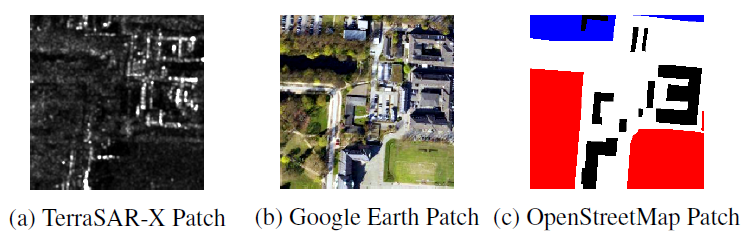
\includegraphics[width=\columnwidth]{dt}
				%		 Create a subtitle for the figure.
			\caption{Image patches from heterogeneous data sources.}
			\label{fig:fw}
		    \hspace{0.5cm}
			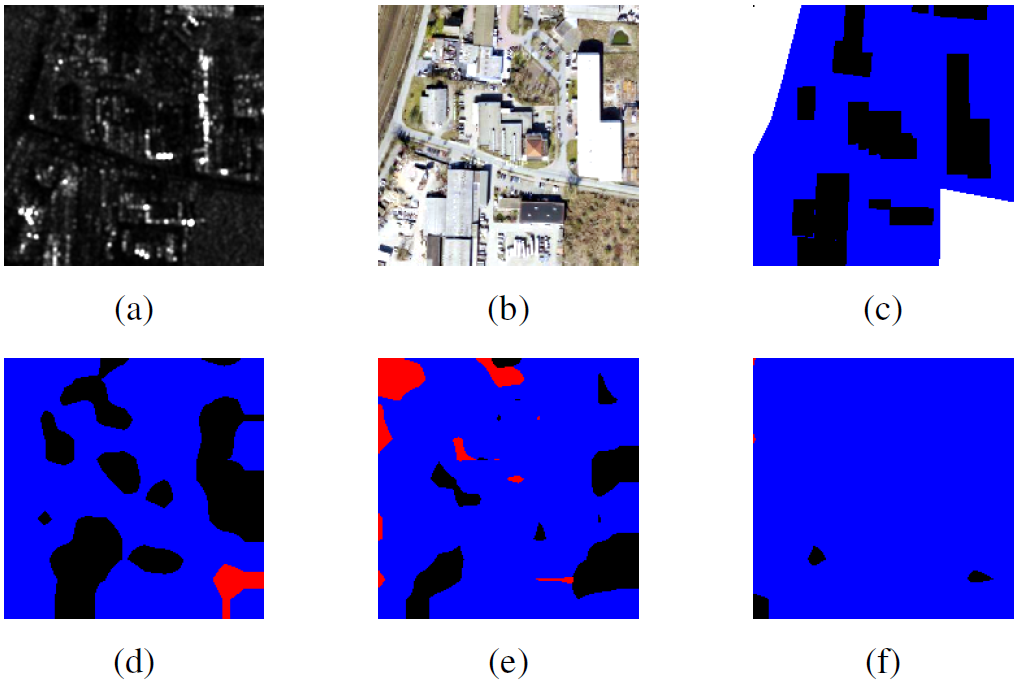
\includegraphics[width=\columnwidth]{rr}
				%Create a subtitle for the figure.
			\caption{Building example of Google Earth Patch Result and TerraSAR-X Patch Result. (a) TerraSAR-X Patch. (b) Google Earth Patch. (c) OpenStreetMap Patch. (d) Google Earth Patch Result with 250 Epochs. (e) TerraSAR-X Patch Result with 750 Epochs. (f) TerraSAR-X Patch Result with 1000 Epochs.}
			\label{fig:rt}
		\end{center}
	\end{figure}

% Now we need a bibliography:
%\begin{thebibliography}{5}
%
%	%Each item starts with a \bibitem{reference} command and the details thereafter.
%	\bibitem{HOP96} % Transaction paper
%	J.~Hagenauer, E.~Offer, and L.~Papke. Iterative decoding of binary block
%	and convolutional codes. {\em IEEE Trans. Inform. Theory},
%	vol.~42, no.~2, pp.~429–-445, Mar. 1996.
%
%	\bibitem{MJH06} % Conference paper
%	T.~Mayer, H.~Jenkac, and J.~Hagenauer. Turbo base-station cooperation for intercell interference cancellation. {\em IEEE Int. Conf. Commun. (ICC)}, Istanbul, Turkey, pp.~356--361, June 2006.
%
%	\bibitem{Proakis} % Book
%	J.~G.~Proakis. {\em Digital Communications}. McGraw-Hill Book Co.,
%	New York, USA, 3rd edition, 1995.
%
%	\bibitem{talk} % Web document
%	F.~R.~Kschischang. Giving a talk: Guidelines for the Preparation and Presentation of Technical Seminars.
%	\url{http://www.comm.toronto.edu/frank/guide/guide.pdf}.
%
%	\bibitem{5}
%	IEEE Transactions \LaTeX and Microsoft Word Style Files.
%	\url{http://www.ieee.org/web/publications/authors/transjnl/index.html}
%
%\end{thebibliography}

% Your document ends here!
\end{document}